%!TEX root = ../Thesis.tex
\chapter{Genetic markers of hub connectivity in the human brain}
\label{ch:Chapter5}
\fancyhead[R]{\textit{Chapter.} \textit{\thechapter: }\textit{Genetic markers of hub connectivity in the human brain}}


% Insert author names, affiliations and corresponding author email (do not include titles, positions, or degrees).

Supplementary materials can be found in Appendix C.

\section*{Preamble}
Preamble text.

\newpage

\section*{Abstract}
Nervous systems characteristically possess a relatively small number of highly connected regions, called network hubs, that are also highly interconnected with each other, forming a so-called `rich-club’. Rich-club organization plays an important role in supporting integrated brain function and is highly conserved, having been identified in diverse species with varying biological complexity. Such conservation points to a potential role of genes in shaping hub connectivity. Here, we comprehensively investigate genetic markers of hub connectivity in the human brain, as measured using diffusion MRI, by characterising its heritability, polygenic basis and transcriptional signature. Using connectome-wide heritability analysis of 117 MZ and 60 DZ twin pairs, we demonstrate that the integrity of connections between hubs are under the strongest genetic control compared to hub-non-hub and non-hub-non-hub connections. Using gene expression data from the Allen Human Brain Atlas, we show that hub regions display a tightly coupled transcriptional profiles, and that this effect is driven by genes regulating energy metabolism, as has previously been shown in the mouse. At the level of structural DNA variation, we demonstrate that higher polygenic liability for psychiatric disorders is associated with reduced structural integrity of hub-hub connections, whereas higher polygenic scores for IQ are related to increased hub connection strength. Together, these findings suggest that connections between hubs are under strong genetic influence, that the genetic variants driving this influence are also implicated in intelligent behaviour and risk for mental illness, and that hub regions are characterised by a distinct and highly conserved transcriptional signature defined by elevated expression coupling of metabolic genes. 

\section{Introduction}

Nervous systems are complex, intricately connected networks that show non-trivial organization over multiple spatial and temporal scales. The underlying wiring principles that lead to this complex organization have however, remained undisclosed. Arguably the longest-standing and most general principles were first proposed by Santiago Ramón y Cajal over a hundred years ago, who stated that neurons and their processes are configured to conserve time, space, and material \citep{RamonyCajal1995}. Conservation of space and material refers to a minimization of cellular and physical resources (e.g., dense cell packing, minimal axonal length) whereas conservation of time refers to the establishment of efficient networks that enable rapid communication between neural elements. 

Since Cajal’s initial proposal, most research has focused on the conservation of space and material. This work has shown that the minimization of network costs, often measured in terms of axonal wiring volume, can explain many features of neuronal organisation \citep{Cherniak1994,Chklovskii2002,Klyachko2003,Rivera-Alba2011,Wen2005}, ranging from the geometry of neuronal arbors \citep{Cherniak1999} to the placement of cortical areas \citep{Cherniak2004}. However, if the connection costs were strictly minimised, nervous systems would resemble a lattice, forming only short-range connections. Several studies have shown this not to be the case. Instead, brain networks possess more long-range connections than would be expected under a pure cost-minimisation model \citep{Bassett2006,Bullmore2012,Kaiser2006}. It is thought that these long-range connections act as shortcuts to facilitate communication between distal brain regions, thereby increasing topological integration within the network \citep{Bullmore2012,Buzsaki2004a,VandenHeuvel2012} and supporting adaptive, functional complexity \citep{Betzel2018}. These considerations suggest that nervous systems are configured to optimize a trade-off between the minimization of wiring cost on one hand and the optimization of communication efficiency, integration and functional complexity on the other \citep{Bullmore2012}. This trade-off is perfectly consistent with Cajal’s conservation laws, such that minimization of wiring costs conserves material and space, whereas minimization of communication delays conserves time. 

A key factor in how nervous systems negotiate the trade-off between conservation of material and time depends on precisely where the long-range connections of the system are formed. Numerous studies of connectomes, acquired in diverse species and measured at different resolution scales, have shown that these long-range connections are preferentially located between highly connected network elements called hubs \citep{Harriger2012,Towlson2013,VandenHeuvel2011,VandenHeuvel2013b}. Indeed, brain hubs are more strongly interconnected with each other than expected by chance, forming a so-called rich club, and the connections between hubs account for a disproportionate fraction of neuronal wiring costs \citep{Arnatkeviciute2018,Fulcher2016,Harriger2012,Towlson2013,VandenHeuvel2011}. Connections between hubs also mediate a large fraction of signal traffic in the brain \citep{Misic2016,VandenHeuvel2011}, indicating that the rich club represents a costly yet central critical communication backbone for the integrated brain functioning \citep{Gratton2012,Markov2013a,VandenHeuvel2018,VandenHeuvel2013a}.Rich-club organisation has been identified in the microscale neuronal connectome of the \textit{C. elegans} \citep{Towlson2013}, the mesoscale connectomes of the mouse \citep{Fulcher2016}, rat \citep{Liang2017}, cat \citep{DeReus2013b}, and macaque \citep{Harriger2012}, and the human connectome as measured at the macroscale with diffusion MRI \citep{VandenHeuvel2011}. This strong conservation of the rich-club organisation across species suggests that genes may play a central role in shaping hub connectivity. 

Several methods are now available to understand how genes shape brain connectivity \citep{Lein2017,Luo2018}. In humans, the three most commonly employed involve (1) quantitative modelling of heritability using twin pairs [for a review see \citep{Jansen2015}], (2) testing for correlations between phenotypic and allelic variation of the genome using either candidate gene, genome-wide, or polygenic associations [for a review see \citep{Thompson2013}]; and (3) testing for associations between network properties and anatomical variations in gene expression using publicly available expression atlases [for a review see \citep{Fornito2019}]. 

Each of these genetic approaches is complementary. Heritability analyses rely on the inherent genetic differences between monozygotic (MZ) and dizygotic (DZ) twin pairs. Assuming that MZ twins share a $100\%$ of their genes whereas DZ twins, on average, share $~50\%$ of their genes, it is possible to use structural equation models to determine the proportion of trait variance that is attributable to genetic factors. Several twin studies have investigated the heritability of various connectivity related phenotypes \citep{Bohlken2014,Colclough2017,Fu2015,Shen2014,Sudre2017}, but none have directly investigated hub connectivity. One small, early study found that cost-efficient properties of functional connectivity in human brain networks were strongly heritable, particularly in areas of association cortex, which are known to be brain network hubs \citep{Fornito2011}. 

One limitation of the twin design is that it does not identify the specific genes or variants that mediate heritability. This limitation can be overcome by testing for associations between trait and allelic variation at multiple alleles scattered throughout the genome. Early candidate gene studies showed poor reproducibility \citep{Hutchison2004,Sullivan2007}, so more recently there has been a major investigation in genome-wide association studies (GWAS) which use very large samples to test for associations at millions of allelic markers throughout the genome \citep{Bush2012}. As an extension of this work, polygenic scores for GWA-investigated traits can be estimated, which aggregate an individual’s net genetic liability for a given phenotype \citep{Torkamani2018}. In the context of brain connectivity, a number of early candidate gene studies found relationships between selected genes and white matter microstructure \citep{Braskie2012,Chiang2011,Jahanshad2012b}, topological network properties \citep{Dennis2011}, and resting state functional connectivity \citep{Filippini2009,Trachtenberg2012,Westlye2011}. Variants related to structural connectivity \citep{Chiang2009,Jahanshad2012a,Jahanshad2013} and a broad set of imaging phenotypes \citep{Elliott2018} have been later identified through the data-driven GWAS. Building on the prior disorder-related GWAS, polygenic scores for a set of psychiatric disorders have been related to cortical gyrification (Liu et al., 2016), functional connectivity \citep{Dezhina2018,Sadeh2018,Wang2017}, and longitudinal changes in white matter properties \citep{Alloza2018}. However, a limitation of this work is that the functional effects of statistically-identified variants may be unclear, and associated variants may not be causal as GWAS can detect an association to a nearby tag variant that does not in itself exert a causal influence on the phenotype \citep{Wang2010}. 

A third approach that more directly bridges the gap between gene function and phenotype relies on recently constructed brain-wide gene expression atlases \citep{Hawrylycz2012} [for a review see \citep{Keil2018}]. Gene expression provide a direct measure of the degree to which a gene has been transcribed in a given tissue and may thus be more proximally related to the functional effects of key genes than statistically-identified DNA variants. However, atlas-based analyses are constructed from post-mortem data, meaning that one can only examine how anatomical variations in the expression patterns of a gene correlate with spatial variations in a given neural phenotype; one cannot understand individual phenotypic variability in this context \citep{Fornito2019}. Moreover, gene expression, commonly quantified through messenger RNA (mRNA) abundance, provides only an indirect marker of the actual abundance of the protein in the cell [\citep{Futcher1999,Greenbaum2003,Gygi1999}, for other limitations of this approach; see \citep{Fornito2019}]. Nonetheless, converging evidence from atlas-based studies suggests that brain network hubs carry a distinct transcriptional signature \citep{Arnatkeviciute2018,Fulcher2016,Rubinov2015c,Vertes2016b}. An initial atlas-based analysis of the mouse connectome found that connected pairs of hubs show increased transcriptional coupling, defined as the similarity in the gene expression profiles between brain regions, relative to hub-non-hub and non-hub-non-hub connections, with the effect being primarily driven by genes regulating oxidative synthesis and metabolism of ATP \citep{Fulcher2016}. Notably, elevated transcriptional coupling of hubs was apparent despite being hubs separated by longer anatomical distances, on average, than other pairs of areas, which showed a strong tendency for reduced transcriptional coupling as a function of anatomical separation. The finding of increased gene expression similarity between hubs also been replicated in the microscale connectome of \textit{C. elegans} nervous system \citep{Arnatkeviciute2018}. Similarly, a separate study of functional connectivity hubs in the human brain found that regions with long connections predominantly linking different modules tend to have higher expression of genes regulating with oxidative metabolism and mitochondrial function \citep{Vertes2016b}. Spatial patterning of gene expression patterns has also been associated with hubs in development \citep{Whitaker2016a} and disease \citep{Rittman2016}. Together, these findings suggest that hub regions across different species and scales exhibit transcriptional properties that are associated with their high metabolic demands. 

Here, we aim to comprehensively investigate genetic markers of hub connectivity by examining heritability, polygenic influences and transcriptional correlates of the macroscale human connectome. We hypothesised that if hub connectivity and rich-club organization is a highly conserved feature of brain organization, then connections between hubs should be strongly heritable. Moreover, if hub connectivity supports integrated function and is susceptible to disease \citep{Crossley2016a,Fornito2015}, then individuals with high polygenic scores for mental illness should show weaker hub connectivity, whereas individuals with high polygenic scores for IQ should show stronger hub connectivity. Finally, given prior findings in the mouse \citep{Fulcher2016} and worm \citep{Arnatkeviciute2018} we predicted that connected pairs of hubs should show elevated transcriptional coupling compared to other areas, and that this effect will be driven by genes regulating metabolism-related processes. 

\section{Materials and methods}

To comprehensively investigate genetic influences on hub connectivity we combine three different data modalities: structural brain connectivity derived from the DWI, brain-wide gene expression atlas data from the AHBA and the polygenic scores for a range of psychiatric disorders and IQ. These rich data allowed us to assess the relationship between brain connectivity and genetics in different ways: quantitatively, through the edge-wise, connectome-wide heritability analysis; at the level of gene expression, through the analysis of the correlated gene expression (CGE) patterns; and at the level of structural DNA variation through polygenic score (PGS) analysis (Figure \ref{fig:Ch5Fig1}). 

\begin{figure}[h!]
\begin{center}
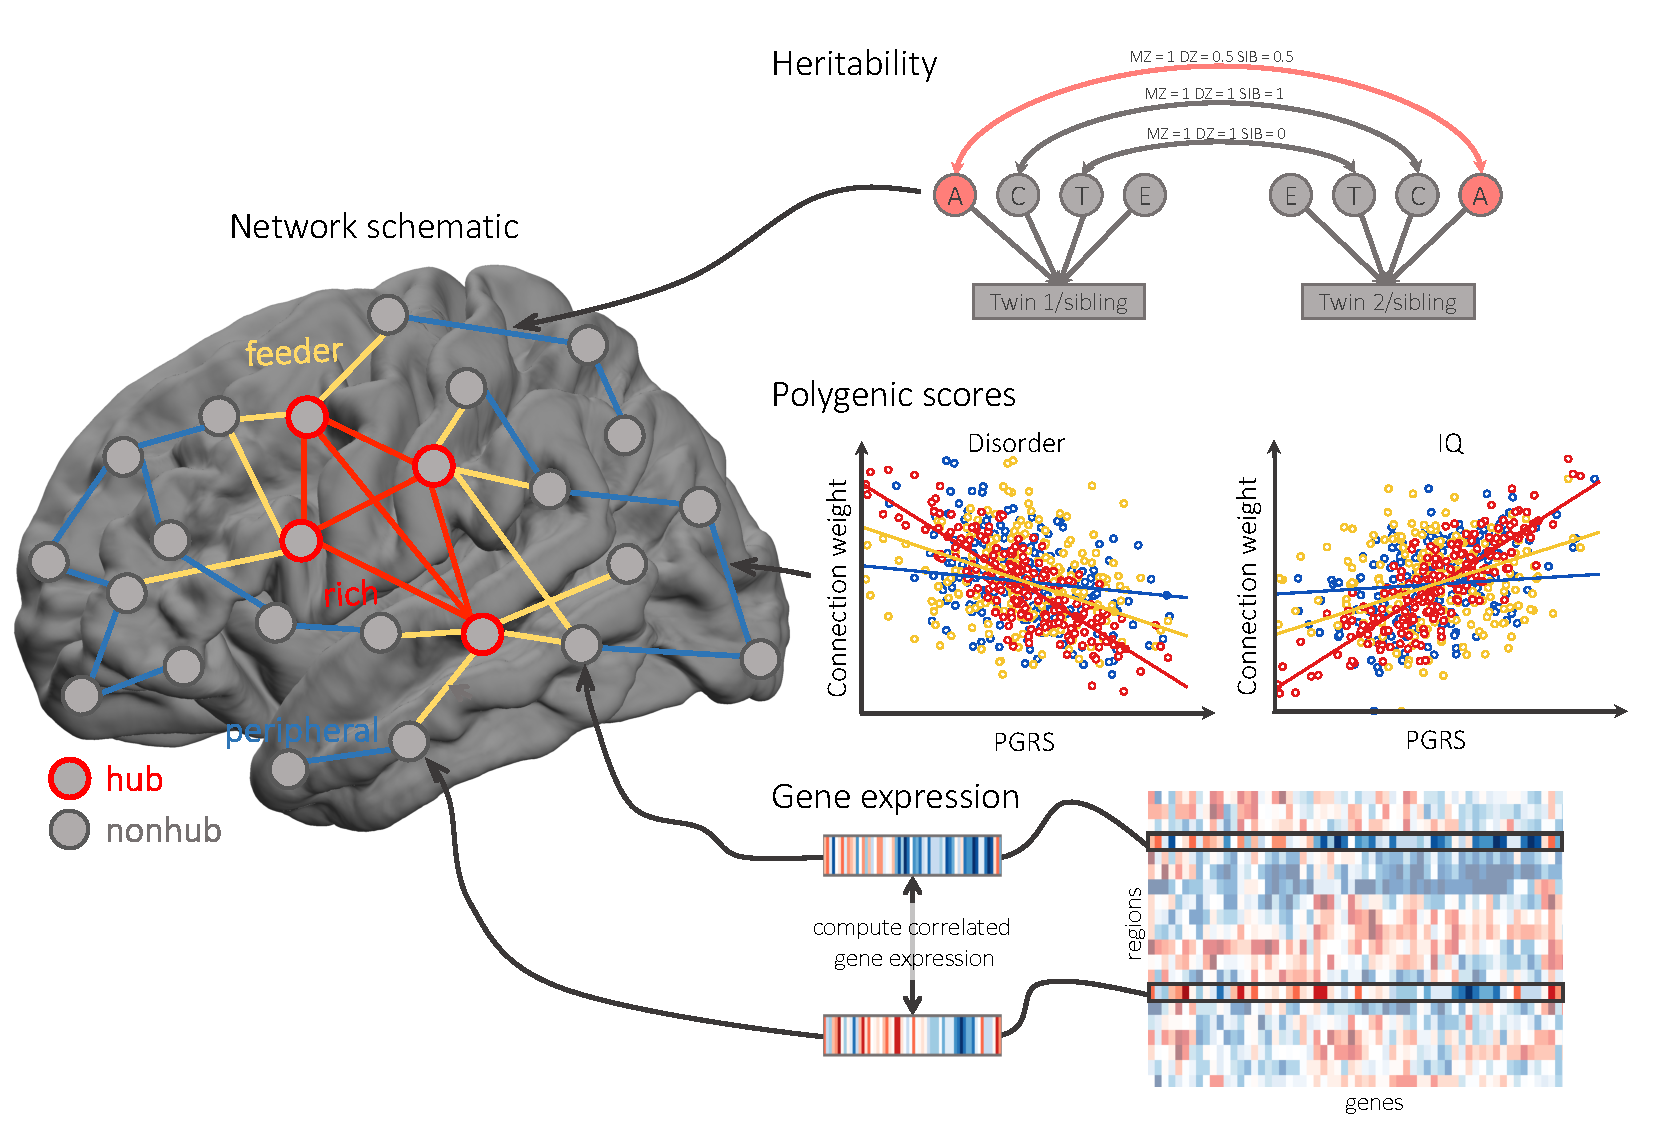
\includegraphics[width=1\textwidth]{Chapter5/Ch5Fig1.pdf}% This is a *.eps file
\end{center}
\caption{\textbf{Investigating the genetic markers of hub connectivity.} 
Left: a schematic representation of the connectome illustrating different connection types in the brain: rich – connections between two hubs; feeder – connections between a hub and a nonhub; peripheral – connections between two nonhubs. Top: heritability analysis using structural equation modelling is applied to every connection within the brain (ACTE model illustrated). Mean heritability estimates are then compared across rich, feeder and peripheral connections; Middle: connection weights for each link across subjects are correlated with polygenic scores for a range of psychiatric disorders and IQ. The average correlation value across link types is then compared between link types. Rich links are expected to show a stronger negative relationship for disorders and a stronger positive relationship for IQ compared to other links within the brain. Bottom: gene expression data from the AHBA is collapsed into a region $\times$ gene matrix. Region-specific vectors of expression values across all genes are then correlated between all pairs of regions, yielding a measure of transcriptional coupling, or correlated gene expression (CGE). Average CGE values are then compared across rich, feeder and peripheral links.}
\label{fig:Ch5Fig1}
\end{figure}

\subsection*{Diffusion weighted imaging}

The DWI data used to define the structural connectivity network were obtained from two separate sources: the Human Connectome Project [HCP, \citep{VanEssen2013}) and a study conducted at Monash University (Monash Cohort). We used the minimally processed DWI and structural data from the HCP for 972 participants ($age_{mean} = 28.7 \pm 3.7$, 522 females), including a cohort of related individuals – MZ and DZ twin pairs together with their non-twin siblings (more details presented in the Heritability section). HCP data were acquired on a customized Siemens 3T ``Connectome Skyra'' scanner at Washington University in St Louis, Missouri, USA using a multi‐shell protocol for the DWI: $1.25 mm^{3}$ isotropic voxels, repetition time (TR) = $5520$ ms, echo time (TE) = $89.5 ms$,  field-of-view (FOV) of $210 \times 180 mm$, $270$ directions with $b = 1000, 2000, 3000 s/mm^{2}$ (90 per b value), and 18 $b = 0$ volumes. Structural T1-weighted data were collected using $0.7 mm^{3}$ isotropic voxels, $TR = 2400 ms$, $TE = 2.14 ms$, FOV of $224 \times 224 mm$. The full details can be found elsewhere \citep{Glasser2013}. 

The Monash Cohort comprised 414 participants with MRI data obtained on a Siemens Skyra 3T scanner at Monash Biomedical Imaging in Clayton, Victoria, Australia using the following DWI parameters: $2.5 mm^{3}$ voxel size, TR = $5520 ms$, TE = $89.5 ms$, FOV of $210 \times 180 mm$, 60 directions with $b = 3000 s/mm^{2}$, and seven $b = 0$ volumes. T1-weighted structural scans were acquired using: $1 mm^{3}$ isotropic voxels, TR = $2400 ms$, TE = $2.14 ms$, FOV of $224 \times 224 mm$. Data for 82 subjects were excluded due to low connectome density ($n = 11$, connectome density more than 3 standard deviations lower than the mean) or no genotype data ($n = 71$), resulting in a sample of 332 participants ($age_{mean} = 23.7 \pm 5.5$, 189 females). 

Pre-processing for T1-weighted structural images in the Monash Cohort consisted of visual screening for gross artefacts followed by the reconstruction of grey/white matter interface and the pial surface using FreeSurfer v5.3.0 software. Surface reconstructions for each subject were visually inspected performing manual corrections if needed in order to achieve a more accurate surface representation. Network nodes for each individual in both datasets were defined using a recently-developed, data-driven group average parcellation of the cortex into 360 regions (180 per hemisphere) \citep{Glasser2016}. To ensure that our results were not driven by the use of this parcellation, we also replicated our findings using a random cortical parcellation consisting of 500 approximately equally sized regions (250 per hemisphere). The advantage of this parcellation is that it minimizes differences in size between regions, which can bias results.

Subsequent processing of the DWI data for both datasets was performed using the MRtrix3 \citep{Tournier2012} and FMRIB Software Library \citep{Jenkinson2012}. Tractography was conducted in each participant's T1 space using second order integration over fibre orientation distributions (iFOD2) – a probabilistic algorithm that improves the quality of tract reconstruction in both highly curved and crossing-fiber regions \citep{Tournier2010}. To further improve the biological accuracy of the structural networks we also applied Anatomically Constrained Tractography (ACT), which delineates the brain into different tissue types (cortical grey matter, subcortical grey matter, white matter, cerebrospinal fluid) and uses that information to ensure streamlines are beginning, traversing, and terminating in anatomically plausible locations \citep{Smith2012}. A total of 10 million streamlines were generated on a probabilistic basis using a dynamic seeding approach that evaluates the relative difference between the estimated fibre density and current streamline reconstruction, and preferentially samples from areas of insufficient density \citep{Smith2015a}. 

The resulting tractogram was then combined with the cortical parcellation for each subject to produce a network map of white matter connectivity. Streamline termination points were assigned to the closest region within a $5mm$ radius. Connection weights were quantified using streamline count (number of streamlines connecting two regions, SC), as well as the mean fractional anisotropy (FA) of voxels traversed by streamlines connecting two regions. Streamline count provides a measure of relative connection strength derived from the tractography algorithm, whereas FA acts as a marker of the white matter integrity along the tract, both measures being subject to certain caveats \citep{Jones2013}. 
Connectomes derived from probabilistic tractography algorithms are often thresholded due to the high probability of false positive connections \citep{Sarwar2019,Sotiropoulos2017}. Commonly used methods involve a range of options including weight-based, consistency-based and density-based thresholding approaches \citep{Betzel2018,Roberts2016a}: weight-based thresholding eliminates connections below a particular threshold; consistency-based thresholding retains connections present in a set proportion of subjects; and density-based thresholding retains connections based on a particular property (weight, consistency or other) to achieve a desired connectome density. No consensus has been reached regarding the most appropriate thresholding method. In our analysis, we combined consistency-based and density-based approaches, such that we selected edges that are commonly reconstructed across subjects and then derived a group-representative connectomes at a selected density. This resulted in a single group-average connectome for the HCP and Monash datasets. Specifically, we: i) selected edges that are present in at least $30\%$ of subjects; and ii) retained the strongest edges (based on the streamline count) to achieve a desired connectome density. Since the desired connection density is arbitrary, we examined our results across a range of densities to evaluate the sensitivity of our findings. For the 360 region parcellation, we considered $15\%$, $20\%$, $25\%$ densities. Given the higher number of possible connections using a higher resolution parcellation of 500 regions, we evaluated slightly lower densities: $10\%$, $15\%$, and $20\%$. 

The group representative connectome derived from the HCP dataset was then used as a binary mask for selecting edges for the heritability and gene expression analyses, while the group representative connectome derived from the Monash dataset was used for selecting edges for the polygenic score (PGS) correlation analyses. We chose to define connections for the gene expression analysis based on the HCP connectomes due to the higher sample size and the superior data quality. In both heritability and PGS analyses, we quantified connection weights using FA and streamline count. We focus on results for the former and present results for the latter in \textbf{Supplementary Material 2}. To enable a more direct comparison to the previous analyses of gene expression in mouse \citep{Fulcher2016} and \textit{C. elegans} \citep{Arnatkeviciute2018}, our gene expression analysis in human was performed using binary connectivity matrices. 


\subsection{Network analysis} 
In this section we outline the network analysis methods that were used to characterize the structural brain connectivity. 

\paragraph*{Degree and strength.}

The connectivity of each region (node) within the network can be quantified by counting the number of connections that a node has, known as degree, \textit{k}. At a particular degree threshold \textit{k}, nodes can be labelled as hubs (degree$>k$) or non-hubs (degree$\leq k$). Subsequently, all the connections within the network can be classified as `rich' (between two hubs), `feeder' (between a hub and a non-hub) and `peripheral' (between two non-hubs). In a weighted network, a node can be also characterised by counting the total weight of its connections, known as node strength. 

\paragraph*{Rich club organisation.}

To quantify the interconnectivity between hub regions within a binary brain connectivity network, we used the topological rich-club coefficient $\phi(k)$:

\begin{equation}
    \label{eqn:Ch5Eq1}
    \phi(k) = \frac{2E_{>k}}{N_{>k}(N_{>k}-1)},
\end{equation}

where $N_{>k}$ is the number of nodes with degree $>k$, and $E_{>k}$ is the number of edges between them \citep{Colizza2006}. Therefore, the rich-club coefficient quantifies the density of the sub-graph consisting of nodes with degree higher than a selected threshold k. Nodes with higher degree make more connections, resulting in a higher expected connection density between them. To quantify levels of connectivity in excess of this, we compared the $\phi(k)$ in the empirical network to the mean value across a 1000 randomized null networks, $\phi_{rand}(k)$, that were generated by rewiring the edges in the empirical network while retaining the same degree sequence, using the \texttt{randmio\_und} function from the Brain Connectivity Toolbox \citep{Rubinov2010}. Each edge on average was rewired 50 times per null network. 

To assess whether the connections between high degree nodes in a weighted network were more likely to have stronger weights than expected by chance, we also evaluated the weighted rich club coefficient \citep{Opsahl2008}: 

\begin{equation}
    \label{eqn:Ch5Eq2}
    \phi^{w}(k) = \frac{W_{>k}}{\sum_{l=1}^{E_{>k}}w^{rank}_{l}},
\end{equation}

where $W_{>k}$ is the sum of weights in the subgraph with degree higher than k and the denominator is the total sum of l strongest weights in the network. Separating the definitions of weighted and topological rich-club coefficients, instead of rewiring the links, here we randomly re-assigned weights within the network while keeping the binary topology of the network the same \citep{Alstott2014}. In both cases, we computed the normalised rich-club coefficient $\phi_{norm}(k)$ as the ratio between the rich-club coefficient in the empirical network and the mean rich-club coefficient in the set of the corresponding randomised networks:
\begin{equation}
    \label{eqn:Ch5Eq3}
    \Phi_\mathrm{norm}(k) = \frac{\phi(k)}{\langle \phi_\mathrm{rand}(k) \rangle}.
\end{equation} 
Values of $\Phi_{norm}$ exceeding 1 indicate rich-club organisation, where high degree nodes are more densely interconnected (in a case of the topological rich-club) or have higher weights (in a case of the weighted rich-club) than be expected by chance. The statistical significance of the result is assessed by computing a p-value directly from the empirical null distribution of the 1000 randomised networks, $\phi_{rand}(k)$, as a permutation test \citep{VandenHeuvel2011}. 

\paragraph*{Communicability.}

Connections that mediate a high proportion of traffic within the brain are critical for information transfer. To confirm that this was the case in our data, and considering that neuronal signals within brain networks may not necessarily propagate along shortest topological paths, we investigated the topological centrality of rich links using a measure of communicability \citep{Estrada2008} across a range of degree thresholds. The communicability (C) between a pair of nodes \textit{i} and \textit{j}, is calculated accounting for all possible paths of length l between the nodes, weighted as $1/l!$, so that shorter paths are assigned higher weights and consequently have a higher contribution to the overall score. The communicability $C_{ij}$ for a binary matrix A is formally defined as: 
\begin{equation}
    \label{eqn:Ch5Eq4}
    C_{ij}= \sum_{l=0}^{\infty}\frac{(A^{l})_{ij}}{l!} = e^{A}_{ij}.
\end{equation} 

\subsection{Heritability analysis} 

The HCP data includes 117 pairs of genetically confirmed monozygotic (MZ) twin pairs together with 82 of their non-twin siblings, as well as 60 dizygotic (DZ) same-sex twin pairs and 58 of their non-twin siblings. For heritability analysis, for each twin pair with more than one non-twin sibling, one sibling was selected at random (demographic details summarized in the \ref{Ch5Table1}). Only twin pairs where both twins had genotyping-verified zygosity were included in the heritability analysis. 

\begin{table}[h!]
\label{Ch5Table1}
\centering
\caption{Demographic data for twin groups and their non-twin siblings. MZ - monozygotic twins, DZ - dizygotic twins. Age is displayed in years: $mean \pm SD$.}
\begin{tabular}{@{}llll@{}}
\toprule
\textbf{Zygosity} & \textbf{Number of subjects} & \textbf{Sex (F/M)} & \textbf{Age} \\ \midrule
MZ twins & 117 pairs & 69/48 & $29.3 \pm 3.3$ \\
MZ non-twin siblings & 69 & 34/35 & $29.1 \pm 4.2$ \\
DZ twins & 60 pairs & 33/27 & $28.8 \pm 3.5$ \\
DZ non-twin siblings & 48 & 24/24 & $29.1 \pm 4.0$ \\ \bottomrule
\end{tabular}
\end{table}

Heritability analysis relies on the assumption that the similarity in a particular trait between twins is due to the additive effects of shared genes or shared environmental factors. While MZ twins share all their genes and therefore are genetically identical, DZ twins on average share half of their genes resulting in $~50\%$ genetic similarity (similar to non-twin siblings). Whereas shared genetic factors as well as common environment contribute to the similarity between twins in a pair, unique environmental factors contribute to the differences observed between them. Therefore, it is possible to decompose the phenotypic variance and covariance in any particular trait into several factors such as additive genetic (A), common environmental (C) and unique environmental (E) influences. Considering that twins raised together might have experienced a more similar environment compared to their non-twin siblings, including a set of non-twin siblings into the analysis allows us to separate the common environmental contributions into twin-specific (T) and twin non-specific (C) common environment. 

Structural equation modelling (SEM) was implemented for every connection in the group-averaged cortical connectome using OpenMx software \citep{Boker2011,Neale2016} in R. The main analysis was performed on the 360 region \citep{Glasser2016} cortical connectome (further referred as f360 parcellation) at $20\%$ density using fractional anisotropy as a connection weight. The analyses were subsequently reproduced with varying connectome densities ($15\%$ and $25\%$) and using a higher resolution random cortical parcellation [500 regions (further referred as r500 parcellation): $10\%$, $15\%$ and $20\%$ densities]. A range of biometric models - ACTE, ACE, AE, CE, E - were implemented in order to find maximum likelihood estimates of additive genetic (A), twin-specific common environmental (T), twin non-specific common environmental (C) and unique environment (E) factors using age and sex as covariates. Outlying connection weight values for each analysis were removed using the boxplot function in R by keeping data points (w) in a range $Q1-1.5 \times IQR< w <Q3+1.5 \times IQR$. The Akaike information criterion (AIC) \citep{Akaike1998} was used to compare the goodness of fit of all tested models in order to find the most parsimonious one. For each edge the model with the lowest AIC was selected. Consequently, the narrow sense heritability [the proportion of variance attributable to additive genetic factors (referred as heritability through this work)] for each connection was estimated as defined by the best-fitting model. 

\subsection{Genotype data} 

DNA samples for 715 individuals of European descent from the Monash Cohort were genotyped using the Illumina Infinium PsychArray-24v1.2 BeadChip at Path West’s Diagnostic Genomics Laboratory in Western Australia. The Illumina Psych-Chip comprising of 510,000 markers: 265,000 tagging SNPs from the Infinium Core-24 BeadChip and 245,000 markers from the Infinium Exome-24 BeadChip. Illumina Psych-Chip was developed in collaboration with the Psychiatric Genomics Consortium (PGC) and supplemented with an additional $~50000$ SNPs implicated in psychiatric and neurodevelopmental disorders. 

We performed quality control (QC) using PLINK 1.9 software at both the individual subject and SNP level. Initially, we removed subjects with very low-genotyping score ($\geq 0.10$ of missing data) and excluded SNPs with genotyping call rate $<90\%$ and with a minor allele frequency (MAF) $< 0.01$. Further, several subject-level QC steps were performed by removing individuals: i) with disparities between the recorded and observed sex status as determined through X-chromosome homozygosity; ii) with low genotyping score ($\geq 0.05$ of missing data); iii) with cryptic relatedness higher than 0.25; iv) displaying outlying mean heterozygosity (greater than $\pm3$ SDs from the sample mean). In order to identify any potential sources of population stratification in the sample we performed multidimensional scaling (MDS) using HapMap3 dataset (Consortium, 2010) and excluded subjects exceeding $\pm±2$SD on the $1^{st}$ or $2^{nd}$ principal components, leaving a total of 666 subjects for the imputation. SNPs with low genotyping call rate $<95\%$, MAF$<0.01$ and significantly departing from Hardy– Weinberg (H–W) equilibrium ($p<10^{7}$) were excluded leaving \num{283 616} variants in the final set taken forward to imputation. We used MaCH and Minimac2 for phasing and genotype imputation respectively employing the 1000 Genomes (phase one release three) reference panel. After imputation, SNPs with MAF$<0.01$ and MAF$>0.98$ were removed. To eliminate poorly imputed variants, SNPs with imputation quality $r^{2} < 0.8$ were excluded resulting in a total of \num{5723894} variants used for the polygenic score calculations. 

\subsection{Polygenic risk score calculation}

Polygenic scores (PGS) for five major psychiatric disorders including schizophrenia, major depressive disorder, ADHD, bipolar disorder and autism spectrum disorder (ASD) and IQ were calculated using PRSice software package \citep{Euesden2015}. The PGS for each subject were estimated as a sum of risk alleles, weighted by their effect size as defined in the latest publicly available GWA study for each trait \citep{Neale2010,Ripke2014a,Ruderfer2018,Savage2018,AutismConsortium2017,Wray2018} while controlling for sex, age, age$^{2}$, age $\times$ sex interaction and four first principal components extracted from the MDS analysis (to adjust for population stratification) as covariates. PGSs are calculated by selecting SNPs based on their association with a trait in the base GWAS. Selecting an appropriate SNP significance threshold for PGS calculations poses an issue of balancing statistical power and the strength of the association with a trait. More stringent thresholds generate a smaller set of SNPs that are more likely to be truly associated with the trait of interest whereas more liberal thresholds might help to increase the statistical power while possessing a risk of selecting SNPs that have weak associations. Considering that we did not have reliable measures of disorder-specific traits in our sample and therefore could not select the most predictive threshold ($p_{T}$) for each disorder, we chose a $p_{T}<0.05$ to balance the statistical power of the estimated PGR and the number of SNPs included in the analyses \citep{Ripke2014a}). The number of selected SNPs varied in the range \num{15 000}-\num{40 000} SNPs, depending on the trait of interest. 

\subsection{PGS correlation}

After selecting the subjects that had both DWI and PGS data available ($n= 332$, $age_{mean} = 23.7 \pm 5.5$, 189 females) we used a partial rank correlation (Spearman) to evaluate the relationship between the connection weight and the polygenic scores for a range of psychiatric disorders (autism, ADHD, major depression, bipolar disorder and schizophrenia) and IQ, while controlling for participant age and sex. For each connection in the representative group connectome defined using the Monash Cohort data, we extracted fractional anisotropy-based connection weight values across subjects (streamline count-based results are presented in the \textbf{Supplementary material 2}). In each correlation, subjects with connections with outlying values were filtered in a two-step procedure: i) only the subjects with an existing connection were retained; ii) among the existing connections, only links with weight (w) within the range of $Q1-1.5 \times IQR< w <Q3+1.5 \times IQR$ were selected, resulting in the median exclusion of 15 subjects ($IQR = 28$) at any individual edge. In the case of SC based connection weights, a median of 36 subjects ($IQR=39$) were excluded at any individual edge. As a result, partial rank correlation coefficients were estimated for every connection in the representative group connectome. 

\subsection{Gene expression}

We used brain-wide gene expression data from the Allen Human Brain Atlas (AHBA), which consists of microarray expression measures in 3702 spatially distinct tissue samples taken from six neurotypical adult brains \citep{Hawrylycz2012}. Different brain regions were sampled across each of the six AHBA donors to maximize spatial coverage, resulting in approximately 400-500 tissue samples in each brain. The samples were distributed across cortical, subcortical, brainstem and cerebellar regions, and quantify the expression levels of over \num{20000} genes. Considering that only two out of six brains were sampled from both right and left hemispheres whereas the other four brains have samples collected only from the left hemisphere, we decided to focus our analyses on the left cortex only. For more details about the data see \citep{Hawrylycz2012}. 

The processing of the gene expression data consisted of several steps, outlined in \citep{Arnatkeviciute2019}. Briefly, i) probe-to-gene annotations were updated using the Re-Annotator toolbox \citep{Arloth2015}; ii) intensity based filtering was applied in order to exclude probes that do not exceed background noise in more than $50\%$ of samples; iii) a representative probe for each gene was selected based on the highest correlation to RNA sequencing data in two of the six brains \citep{Miller2014a}; iv) gene expression samples were assigned to the regions-of-interest by generating donor-specific grey matter parcellations and assigning samples located within 2mm of the parcellation voxels; v) gene expression measures within a given brain were normalised first by applying a scaled robust sigmoid normalisation [see \citet{Arnatkeviciute2019}] for every sample across genes and then for every gene across samples in order to evaluate the relative expression of each gene across regions, while controlling for donor-specific differences in gene expression [see \citet{Arnatkeviciute2019} for a validation]. Normalised expression measures in samples assigned to the same region were averaged within each donor brain and aggregated into a region by gene x matrix consisting of expression measures for \num{10027} genes over 180 (left hemisphere, HCP parcellation) and 250 regions (left hemisphere of the random parcellation) respectively. For more details, see the \textbf{Supplementary material 1}. 

\subsection{Transcriptional coupling}

Using the brain-wide gene expression measures derived from the AHBA we quantified transcriptional coupling between regions using the measure of correlated gene expression (CGE). We defined CGE as the Pearson correlation between the normalized expression measures of available genes after pre-processing ($n=\num{10027}$). As shown in Figure \ref{fig:Ch5Fig1} and described in \citep{Arnatkeviciute2019}, CGE exhibits a strong spatial autocorrelation that can be approximated by an exponential relationship, where pairs of regions in close proximity to each other demonstrate much more similar expression patterns (higher CGE) compared to region pairs separated by longer distances. To investigate whether CGE differs between different topological classes of connections beyond any low-order spatial effect, we fit an exponential function with form $r(d)=Ae^{-d/n}+B$. The parameters $A = 0.64$, $B = -0.19$ and $n=90.4$ capture the trend well, allowing us to retain the residuals for further analysis (Figure \ref{fig:Ch5Fig2}), defined as $\widehat{CGE_{ij}}=CGE_{ij} - r(d_{ij})$. These distance-corrected residual CGE values were used in all CGE analyses. 

\begin{figure}[h!]
\begin{center}
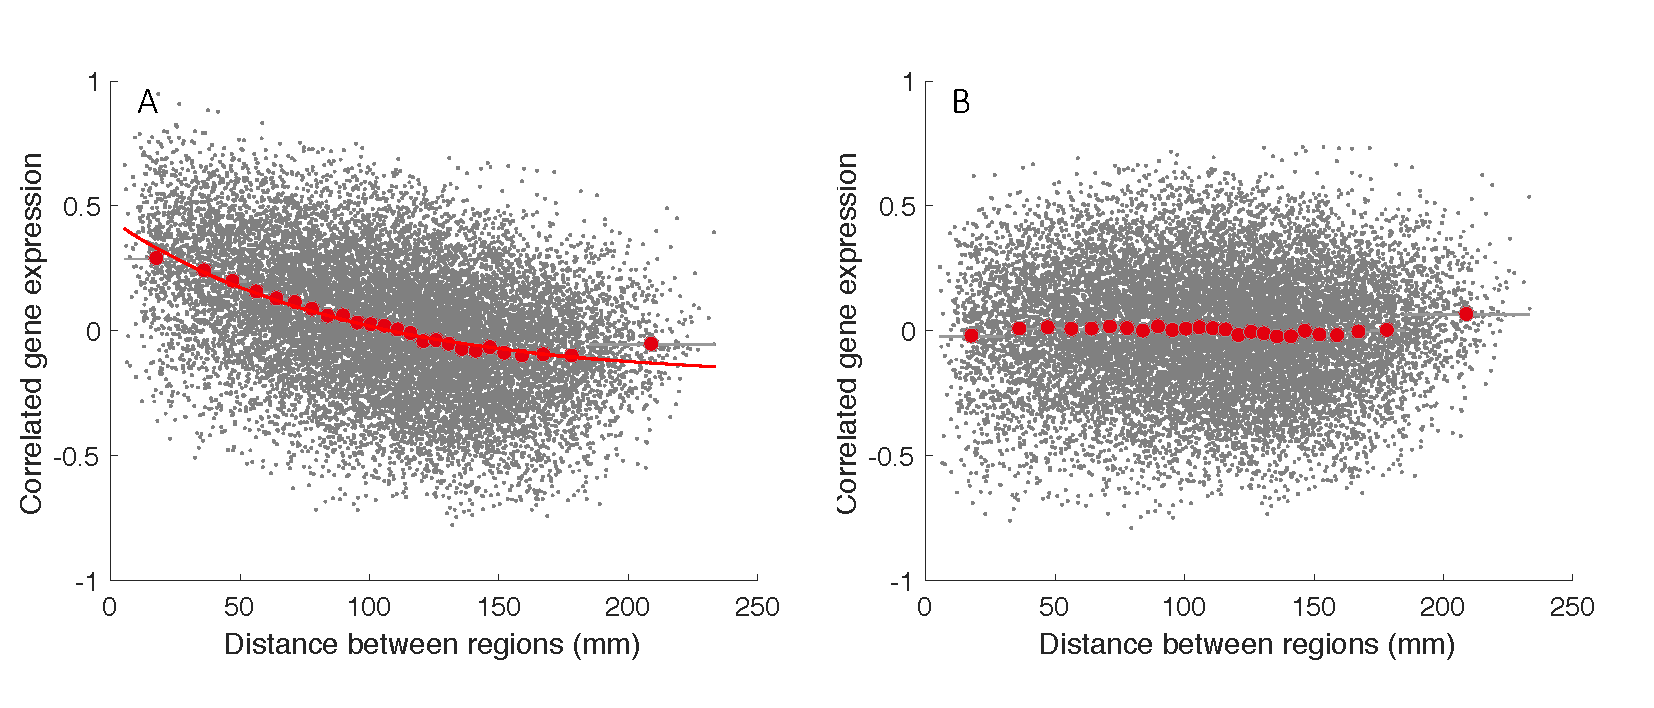
\includegraphics[width=1\textwidth]{Chapter5/Ch5Fig2.pdf}% This is a *.eps file
\end{center}
\caption{\textbf{Relationship between the correlated gene expression and regional separation distance.} 
A) Correlated gene expression as a function of the regional separation distance on the cortical surface. The red line represents an exponential fit $r(d)=0.64e^{-d/90.4}-0.19$. B) CGE residuals after removing the exponential trend. CGE between pairs of regions are represented in grey dots and red dots represent the mean value in 25 equiprobable distance bins.}
\label{fig:Ch5Fig2}
\end{figure}

To evaluate transcriptional coupling between different connection types, for every edge within the connectivity matrix, we assigned a distance-corrected CGE measure. At each degree threshold \textit{k} for defining hubs (degree$>k$) we then computed an average CGE value for every link type (rich – connection between two hubs, feeder – connection between a hub and a nonhub and peripheral – connection between two nonhubs). Significant increases in the CGE for a given link type compared to the rest of the network were evaluated using a one-sided Welch’s t-test ($P<0.05$). 

To determine which functional gene groups contribute the most to any observed differences in CGE across different link types in the brain, we estimated the gene contribution scores (GCS) as previously shown in \citep{Fulcher2016} using the definition of the Pearson correlation coefficient: 

\begin{equation}
    \label{eqn:Ch5Eq5}
    \widehat{CGE_{ij}} = CGE_{ij} - r(d_{ij}) = \frac{1}{N}\sum_{a=1}^{N}[\widetilde{g}_{i}^{a}\widetilde{g}_{j}^{a} - r(d_{ij})],
\end{equation} 
where N is the number of genes (N = \num{10 027}), $\widetilde{g}_{i}^{a} \widetilde{g}_{j}^{a}$ the product of the z-score normalised expression values for a gene \textit{a} in regions \textit{i} and \textit{j} and $r(d_{ij})$ is a previously defined spatial autocorrelation effect approximated as an exponential line. Therefore, the gene contribution score between a pair of regions i and j for a gene a was defined as $GCS_{ij}^{a}= \widetilde{g}_{i}^{a}\widetilde{g}_{j}^{a} - r(d_{ij})$.

We then assigned each gene a t-statistic quantifying the increase in GCS for rich compared to peripheral links, as these two groups constitute the most distinct link types: a high value indicates a more correlated gene expression pattern among rich compared to peripheral links. Those t-statistic measures were then used in the enrichment analyses as gene scores for determining whether any functional gene groups were contributing more than others. 

\subsection{Enrichment analysis}

The gene enrichment analyses are designed to assess whether any functional gene groups are overrepresented in a large set of genes. Every gene in our sample (n= \num{10027} genes) was assigned a t-statistic score quantifying its contribution towards the increase in GSC for rich links. Using these scores we aimed to determine which specific functional groups of genes contribute to the observed increase in correlated gene expression. Functional gene group analysis was performed using version 3.1.2 of ErmineJ software \citep{Gillis2010}. Gene ontology (GO) \citep{Ashburner2000} annotations were obtained from GEMMA \citep{Zoubarev2012} as \texttt{Generic\_human\_ncbiIds\_noParents.an.txt} on May 16, 2018. Gene Ontology terms and definitions were acquired from the \url{archive.geneontology.org/latest-termdb/go_daily-termdb.rdf-xml.gz} on May 16 2018. We performed gene score resampling (GSR) analysis on the t-statistic scores testing the biological process GO categories with 5 to 100 genes available using the mean t-statistic score across genes to summarise the GO category and applying full resampling with 106 iterations. Resulting p-values were FDR-corrected across \num{5987} GO categories using the false discovery rate method of Benjamini and Hochburg \citep{Benjamini1995}.
  